\documentclass[workingdraft]{usetex-v1}

%% For intial submission uncomment the following code to remove ednote
%% comments

%\makeatletter{}
%\newsavebox{\kfl@discard}
%\renewenvironment{ednote}[1]{\@latex@warning
%  {Leftover ednote environment in final version ignored}%
%  \begin{lrbox}{\kfl@discard}}{\end{lrbox}}
%\makeatother{}

\usepackage{preamble}


% Hacks
\setcounter{secnumdepth}{1}
\newcommand*{\andshare}{\end{tabular}\\\begin{tabular}[t]{c}}



\begin{document}

\title{mGTK: An \sml binding of \gtk\\\relax[Extended Abstract]}

\docstatus{Submitted to USENIX'04 (FREENIX track)}

\author{
\authname{Ken Friis Larsen}
\authurl{\url{ken@friislarsen.net}}
\and
\authname{Henning Niss}
\authurl{\url{hniss@it.edu}}
%
\andshare{}
\authaddr{Department of Innovation}
\authaddr{IT University of Copenhagen}
\authaddr{Denmark}
%
} % end author

\maketitle

\DefineShortVerb{\!}

\begin{abstract}
  We describe \mgtk, a Standard ML language binding for the \gtk
  toolkit.  \gtk is a graphical toolkit for the X Window System, and
  provides an object-oriented C language API.  Since Standard~ML is a
  mostly-functional language without object types, constructing a
  binding to \gtk is not a trivial task.  This paper describes
  how it is possible to encode a single-inheritance class-hierarchy
  using \sml's type system. And we describe how we machine-generate
  most of the binding to best utilize the limited man-power of the
  project.  

  \begin{ednote}{Bart}
    You will also want to add a few sentences, describing the
  rest of the paper contents, and describing impacts and contributions
  of the work.
  \end{ednote}

\end{abstract}



\section{Introduction}
\label{sec:intr-backgr}

This section gives a brief introduction to \sml and \gtk, and presents
an overview of the rest of the paper.

\textit{[Note to PC: We decided to remove some motivation and background
  in favor of an introduction to \sml; in the final version we expect
  to start out with motivation and background.]}

\begin{ednote}{Ken}
  We need to motivate and explain why it is interesting with a GUI lib
  for SML.  That should be easy:  Because there currently isn't (a
  standard industrial strenght) one.  On a long term basis,
  when we have wrapped the whole GNOME platform, it is possible to SML
  to make real applications without inventing the weel to many times.

  Second we need to explain why an SML binding is interestinf from a 
  GTK point-of-view: Opens up the small, but important, marked of
  teaching languages; tests the interfacability of GTK, as SML is
  radically different than C (and most other mainstream languages). 
\end{ednote}

\subsection{Standard ML}

\begin{ednote}{Ken}
  Take one.  It is crap but is it here
\end{ednote}

Standard ML (\sml) is a functional language with imperative features
widely used for teaching and in research.  It is roughly on the same
level of abstraction as Python or Scheme. In contrast to Python and
Scheme, which are \emph{dynamically typed}, \sml is \emph{statically
  typed} (like Java and C++) which means that type errors are detected
at \emph{compile time} rather than at \emph{run time}.  Despite \sml
being statically typed, it is not necessary for the programmer to
explicitly provide type annotations in the program. \sml features
\emph{type inference} which means that the compiler reconstructs type
annotations as needed.

\sml is one of the few languages with a formal definition
\cite{Milner:1997:Definition}.  The definition defines \sml in 93
pages of mathematical notation (a "big step" structured operational
semantics, plus type inference rules) and English prose.  The book is
not meant as tutorial for the language. Rather, it provides an
implementation-independent formulation of \sml.  This formal
definition means that it is possible to write substantial applications
in \sml that are not dependent on a specific compiler.  There are also
several mature \sml implementations with widely different
implementation strategies ranging from byte-code interpreters with
interactive \emph{read--eval--print--loops} (REPLs) to aggressively
optimizing whole-program compilers targeting native code.




\subsection{\gtk}
\label{sec:gtk}

\gtk (GIMP Toolkit) is a library for creating graphical user
interfaces. It is licensed using the LGPL. It is the graphical toolkit
used in the \gnome platform.  \gtk is implemented in C, but from the
beginning the \gtk developers have paid attention to making it feasible
and practical to develop bindings for other programming languages than C.

\begin{ednote}{Bart}
  "...is a library...It is licensed...LGPL..." -> "is an
  LGPL-licensed [cite LGPL] library for creating..."  i.e, fold
  second sentence in to first, and add LGPL cite.
\end{ednote}

\begin{ednote}{Bart}
     "It is the graphical toolkit used in the GNOME platform."  Add more
   sentences to this to make a paragraph with a brief history of
   GIMP/GNOME/Gtk/Gtk+.
\end{ednote}

\begin{ednote}{Bart}
     "...than C."  Should section 4 material move here to
   describe the gtk.defs file?

\end{ednote}


%\subsection{Overview of this paper}
%\label{sec:overview-this-paper}



\section{Brief Introduction to \sml{}}
\label{sec:brief-intr-sml}

This section gives a breif overview of some of the main features of
\sml{}.  It is not enough to use the language in anger, but it should
be sufficient to get an understanding of the examples in the rest of
the paper.  We refer the interested reader to one of the fine textbooks
\cite{Hansen-Rischel:1999,Paulson:1996} for more information about \sml{}.

\begin{ednote}{HN}
I don't like the sentence ``\ldots use the language in anger'' (what
does this ``anger''-thing mean?).
\end{ednote}

\sml{} is a two-level language, it consists of a \emph{core language}
for programming in the small (that is, functions, data structures and
algorithms), and a \emph{module language} for programming in the large.


\begin{figure*}[thp]
\mbox{}\hfill{}

\begin{subfloat}
\begin{minipage}[b]{.46\linewidth}
\begin{verbatim}
signature STACK = sig 
  type 'a stack
  exception EmptyStack
  val empty : 'a stack
  val push  : 'a * 'a stack -> 'a stack
  val pop   : 'a stack -> 'a * 'a stack
end
\end{verbatim}
\end{minipage}
\caption{\label{fig:stack-sig}interface}
\end{subfloat}
\qquad
\begin{subfloat}
\begin{minipage}[b]{.46\linewidth}
\begin{verbatim}
structure Stack :> STACK =
struct
  datatype 'a stack =
           Empty
         | Stack of 'a * 'a stack
  exception EmptyStack
  val empty = Empty
  fun push(elem, stack) = 
      Stack(elem, stack)
  fun pop stack =
      case stack of
          Empty => raise EmptyStack
        | Stack(top, rest) => 
          (top, rest)
end
\end{verbatim}
\end{minipage}
\caption{\label{fig:stack-struct}implementation}
\end{subfloat}
\hfill\mbox{}
\caption{Simple stack library implemented in SML.}
  \label{fig:stack-lib}
\end{figure*}

Figure~\ref{fig:stack-lib} show a small stack library implemented in
SML.  This example shows most of the important features of SML.  The
library consists of two parts: an interface description, which is
called a \emph{signature} in SML (Figure~\ref{fig:stack-sig}), and an
module implementation, which is called a \emph{structure} in SML
(Figure~\ref{fig:stack-struct}).  Informally speaking, a
signature is the type of a structure. It specifies the
declarations of the structure that is to be visible from the outside.


The signature is named !STACK!, its extent is delimited by
\texttt{sig} \ldots\ \texttt{end}, and it contains five
specifications: one type specification, one exception sprcification,
and three value specifications.

The type specification !type 'a stack! states that a module that
satisfy (implements) the signature !STACK! must declare a type named
!stack! and that this type is parameterized.  The !'a! is a \emph{type
  variable} and this is what makes the type parameterized.  Type
variables can be instansiated to other types.  Thus, the type of a
stack of intergers is !int stack!, the type of a stack of integer
stacks is !int stack stack!, and so on. Type variables are the core of
\emph{parametric polymorphism} (also known as generics in, for
example, C++ and Java; see \cite{garcia03:generics} for a comparison
of programming languages with support for parametric polymorphism).
The type specification does not say anything about how a stack must be
implemented.

The exception specification just states that an exception named
!EmptyStack! must be declared.

The first value specification says that a constant named !empty! must
be declared and that this constant must have type !'a stack!.  That
is, !empty! is a \emph{polymophic} value, it can be used in contexts
where an \texttt{int stack} is needed or in contexts where a
!int stack stack! is needed.  The next value specification states that a
function named !push! must be implemented, and that this function
takes two arguments: an element and a stack, and returns a stack.
Again, we see how type variables are used to specify that !push! must
work with stacks where the elements can have any type.  The last value
specification states that a function named !pop! must be implemented,
and that !pop!  takes a stack as argument and returs an element and a
new stack.

Figure~\ref{fig:stack-struct} show the code of the implementation, that is a
structure declaration.  The declarations states
that the structure is named !Stack!, that !Stack! satisfies the
signature !STACK!, and that !Stack! does not reveal any implementation
details not revealed by !STACK! (that is what the !:>! means).  The
extent of a structure is delimited by \texttt{struct} \ldots\ 
\texttt{end}.

The parameterized type !stack! is implemented by an algebraic data
type, that is, the !datatype! declaration.  This declaration says that
an !'a stack! is either: the constant !Empty! or constructed by
applying the constructor !Stack! to an element and a stack (constants
declared by a !datatype! declaration, such as !Empty!  is sometimes
called unit constructors or just constructors).

The exception declaration !exception EmptyStack! just declares an
exception.

The next declaration just states that !empty! is bound to !Empty!.  The
function !push! just applies the constructor !Stack! to its argumets.
The function !pop! is more interesting, it takes a stack as argument
(here we have reused the name !stack! as types and values uses
different namespaces, thus the same name can be used for both a type
and a value) and then uses a !case! expression to analyse its argument.
If the argument is the empty stack (the constant !Empty!) then the
exception !EmptyStack! is raised (thrown); otherwise, if the argument
has been constructed with !Stack! applied to the arguments !top! and
!rest! then a pair consisting of !top! and !rest! is returned.

Now, users of this library can call functions from the structure
!Stack! by using ``dot-notation'', for example !Stack.pop mystack!.

This small example illustrate one of the cornerstones in functional
programming, namely that new values are constructed by analyzing,
composing, and sharing old values, in contrast to imperative and
object-oriented programming where values are copied and modified
(although, a new trend in object-oriented programming is to simulate a
functional style, see for example \cite[Item 13 and
14]{bloch01:effective-java}.





%  \sml also features algebraic
%datatypes, pattern-matching, tuples and records, first-class and
%anonymous functions, exception handling, immutable data types and
%updatable references, abstract data types, and parametric modules, but
%it is outside the scope of this paper to introduce all these features,
%instead 





\section{``Hello World'' in \mgtk}
\label{sec:example}

Figure~\ref{fig:hello-world} shows a deliberately simple ``Hello World''
example using \mgtk. It illustrates (1) how to get the toolkit
initialized using \texttt{GtkBasis.init} (from a module containing
basic \gtk functionality not related to specific widgets), (2) how to
construct new widgets (using module \texttt{Window} for the Window
widget, and \texttt{Button} for the Button widget), and (3) how to
connect signals to widgets (using module \texttt{Signal}).
\begin{figure*}[htp]
\begin{centering}
\begin{verbatim}
structure HelloWorld = struct
  fun hello _ = print "Hello World\n"

  fun main _ =
      let val _ = GtkBasis.init(CommandLine.name()::CommandLine.arguments())
          val window = Window.new ()
          val button = Button.new_with_label "Hello World"
      in  Signal.connect window (Widget.delete_event_sig (fn _ => false))
        ; Signal.connect window (Widget.destroy_sig GtkBasis.main_quit)
        ; Signal.connect button (Button.clicked_sig hello)
        ; Container.add window button
        ; Widget.show_all window
        ; GtkBasis.main() 
      end
end

val _ = HelloWorld.main()
\end{verbatim}
\caption{Hello World in \mgtk.\label{fig:hello-world}}
\end{centering}
\end{figure*}

In the figure we use the following \sml constructs not explained
earlier: \texttt{fn}
\textit{x} \texttt{=>} \textit{exp} denotes a similar \emph{anonymous}
function. If one does not care about the parameter, one can use the
\emph{wildcard} \texttt{\_}. The construct \texttt{let}~\texttt{val}
\textit{x} \texttt{=} \textit{exp} declares the identifier \textit{x}
to be bound to the value obtained by evaluating \textit{exp}. If the
only reason for evaluating \textit{exp} is any potential side effect,
one can again use the wildcard \texttt{\_}. Expressions evaluated for
their side effects only can also be sequentialized using \texttt{;}.
The value \texttt{()}, ``unit'', can be used as is and is also used as
the return value of purely side-effecting functions.  Finally,
\texttt{::} denotes the cons operation on lists as in
\textit{hd}\texttt{::}\textit{tl}.


\begin{ednote}{Bart}
     Give the anonymous lambda a name, so that you don't have to explain
   => and so it's obvious what it does.  The non-SML reader can probably
   most easily (and fairly harmlessly) think of the unit value as the
   nullary tuple.  Note that :: is the module operator in C++ and
   friends; you might want to mention that things are different here.

   Explicitly say at some point that "The type of an object in
   a programming language is defined by the set of values it
   can contain."  This makes the par on base types clearer in
   my opinion.

   Give examples of building up derived types from base types:
   in particular, you need to talk about type definitions
   explicitly sometime before section 3.

\end{ednote}


%% Example base types are {\tUnit} for the unit value \texttt{()},
%% {\tInt} for integer values, and {\tBool} for boolean values. The type
%% of a list of integers is \tList{\tInt}. The type of a function
%% expecting an integer list argument and returning an integer result is
%% \tArrow{(\tList\tInt)}{\tInt}; the \textit{length} function on lists
%% would have such a type, for example. 

%% Some functions never need to
%% ``inspect'' (sub)parts of supplied arguments values; such functions
%% are called \emph{polymorphic}. For example, the function that just
%% returns it's argument unchanged (the ``identity function'') is
%% polymorphic; so is the function that computes the length of a list. We
%% indicate the parts of the values that are not inspected by using type
%% variables $\alpha, \beta, \ldots$ at the corresponding locations in
%% the type. For example, the type of the identity function is
%% $\tArrow{\alpha}{\alpha}$ telling us that we can apply it to any type of
%% argument, and we get back a value of the same type. The
%% \textit{length} function has type $\tArrow{\tList\alpha}{\tInt}$
%% because, regardless of the type of elements in the list (here denoted
%% $\alpha$), the function can compute the length of the list. Such type
%% variables are \emph{instantiated} to (more) specific types when we
%% apply the polymorphic function. For example, when we apply the
%% polymorphic identity function to \texttt{()} we instantiate $\alpha$
%% to {\tUnit} giving this occurrence of the function the type
%% \tArrow\tUnit\tUnit; when we apply it to \texttt{17} we instantiate
%% $\alpha$ to {\tInt} and the occurrence of the function gets type
%% \tArrow\tInt\tInt. The function is said to be (parametric) polymorphic
%% because we can apply it to arguments of many shapes.

%% Some functions never need to
%% ``inspect'' (sub)parts of supplied arguments values; such functions
%% are called \emph{parametric polymorphic}. For example, the 
%% function \textit{length} that computes the length of a list is polymorphic. We
%% indicate the parts of the values that are not inspected by using type
%% variables $\alpha, \beta, \ldots$ at the corresponding locations in
%% the type. Then the type of \textit{length} is
%%  $\tArrow{\tList\alpha}{\tInt}$
%% because, regardless of the type of elements in the list (here denoted
%% by $\alpha$), the function can compute the length of the list. Such type
%% variables are \emph{instantiated} to (more) specific types when we
%% apply the polymorphic function. For \textit{length}, when we
%% apply it to a list of booleans we instantiate $\alpha$
%% to {\tBool} giving this occurrence of the function the type
%% \tArrow{\tList\tBool}\tInt; when we apply it to a list of
%% integers  we similarly instantiate
%% $\alpha$ to {\tInt}.

\section{Encoding of Classes}
\label{sec:encoding-classes}

As described in Section~\ref{sec:intr-backgr}, \sml in is a functional
language without object-oriented features and \gtk is designed as an
object-oriented library.  Thus, it is not easy to see how to make an \sml
interface to \gtk.  The most difficult problem is how to present the
subtype relations defined by a class hierarchy in \sml's type system.
That is, in this section we are only interested in how to present a
type-safe \sml interface to \gtk class hierarchy.  By \emph{type-safe} we
mean that, if an \sml application programmer uses our library and
makes a type-error when using the \gtk library, calling a undefined
method on object, for instance, then the \sml compiler should give an
type error (at compile-time).


\begin{ednote}{Bart}
  Explain in a few sentences why OO class hierarchies can be
  thought of as having a subtype relationship.  Believe it or
  not, this won't be obvious to everyone.
\end{ednote}

Fortunately, we are able to take advantage of two properties of \gtk
and \sml.  First, \gtk implements a class system with only
single-inheritance.  Second, \sml's type system is expressive enough
to express the subtype relations of single-inheritance class
hierarchies.  



In type theoretical jargon, the trick is to use parametric
polymorphism and \emph{existential types} to encode inheritance
subtyping.  In particular we use \emph{phantom types} to encode the
inheritance path.


\begin{figure}[htp]
  \centering
% 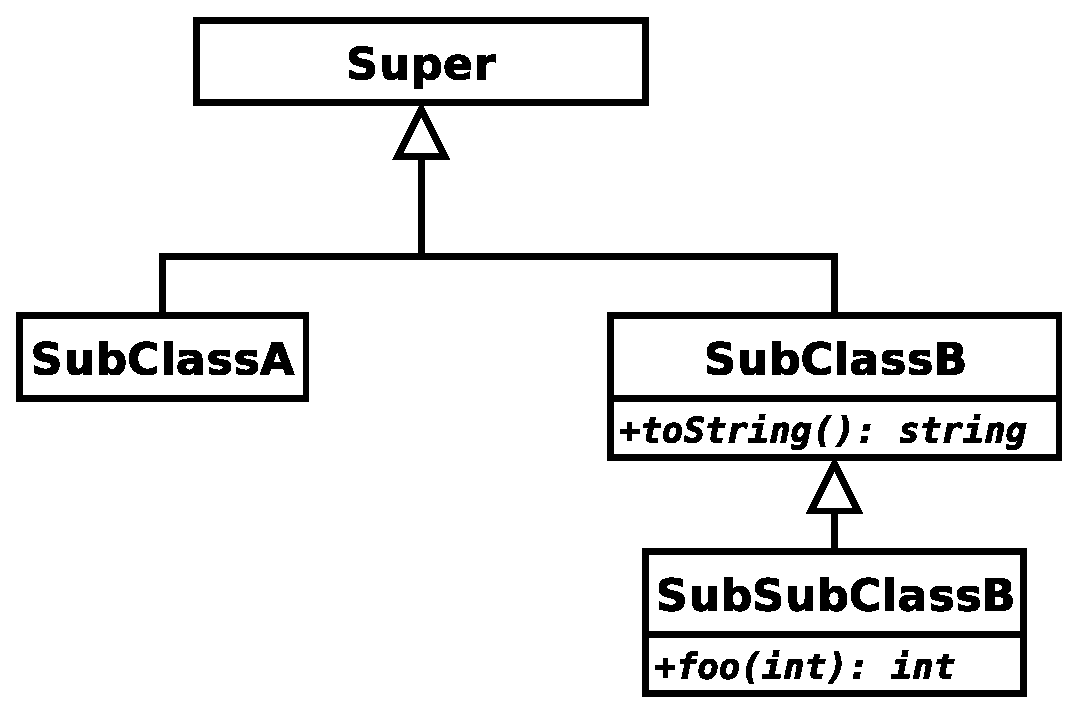
\includegraphics[width=.8\linewidth]{example-class-diagram.eps}
%  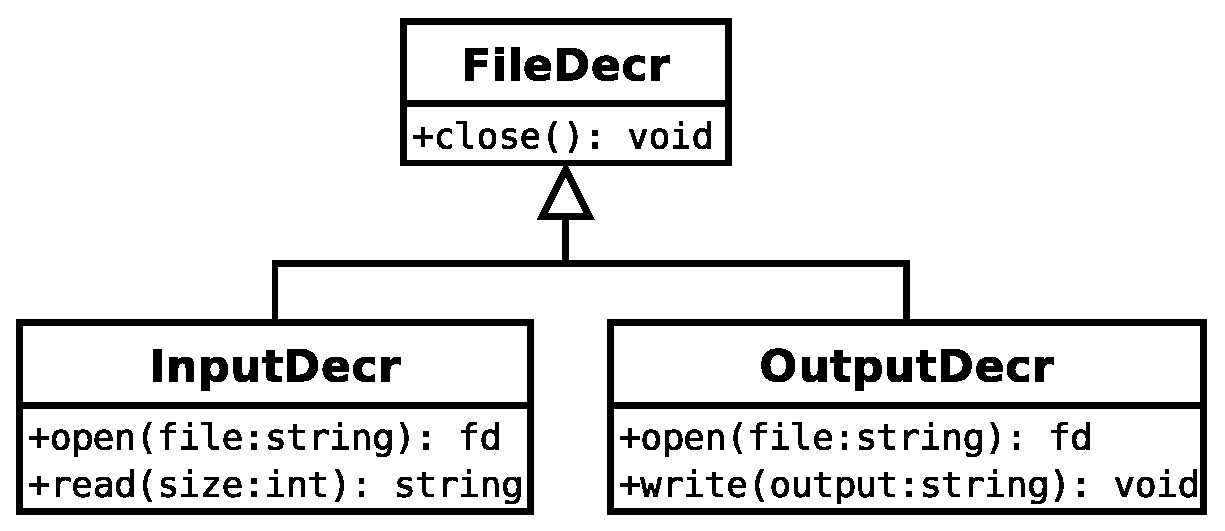
\includegraphics[width=.8\linewidth]{filedecr-class-diagram.eps}
  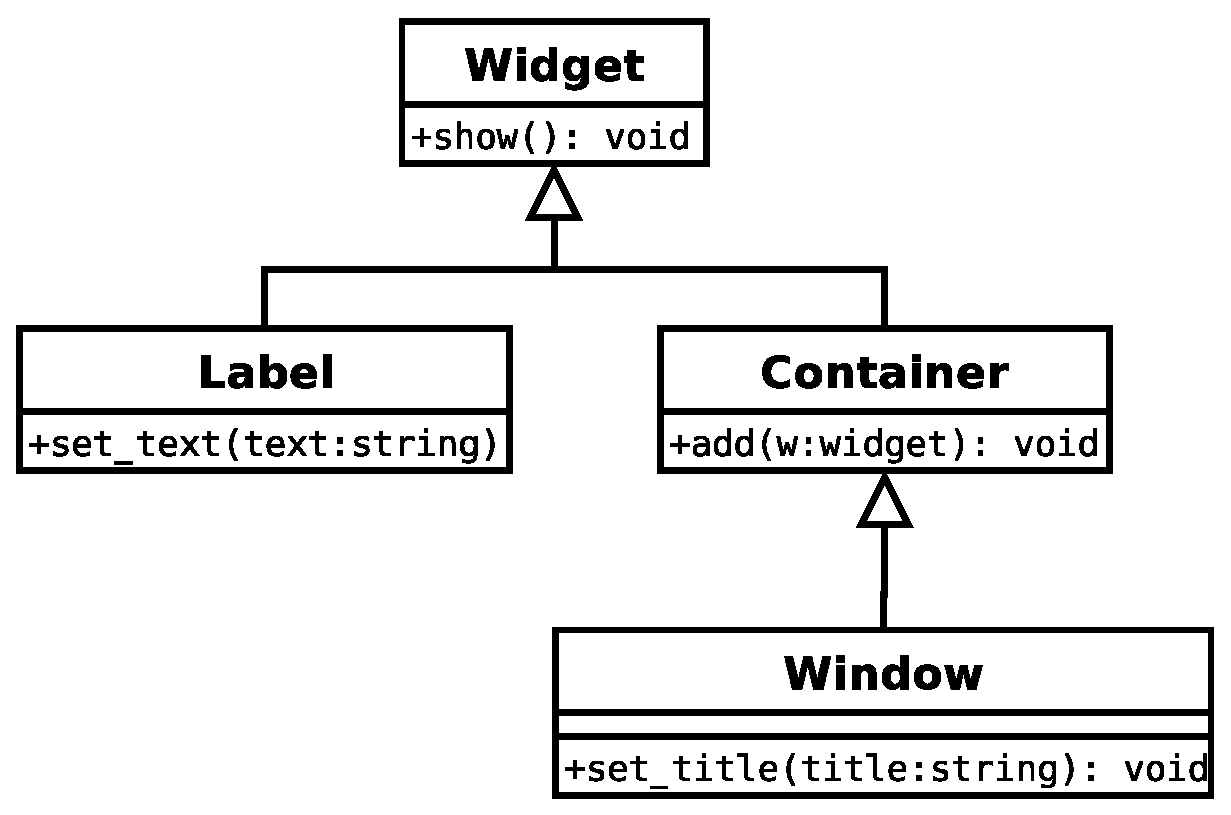
\includegraphics[width=.9\linewidth]{widget-class-diagram.mps}
  \caption{Small example class hierarchy}
  \label{fig:class-hierarchy}
\end{figure}

Figure~\ref{fig:class-hierarchy} shows a small class hierarchy with
just four classes. \classname{Label} and \classname{Container} are
subclasses of the class \classname{Widget} and \classname{Window} is a
subclass of \classname{Container}.  We shall go through the different
parts of the encoding of a class.  For the specific class hierarchy i
Figure~\ref{fig:class-hierarchy}, the properties we want from our
type encoding into \sml's type system to enforce is that we should be
allowed to call the !show! method on all kinds of arguments whether
they are of class type \classname{Widget}, \classname{Label},
\classname{Container}, or \classname{Window}; we should be allowed to
call the !add! method on \classname{Container}s and
\classname{Window}s, but not \classname{Widget}s and
\classname{Label}s; we should only be allowed to call !set_title! on
\classname{Window}s; and so on. 


\begin{description}
\item[Class types] A base class like \classname{Widget} in
  Figure~\ref{fig:class-hierarchy} is encoded as an abstract
  parameterized type:
\begin{SMLcode}
type 'path super
\end{SMLcode}
(we follow the convention suggested by the \smlbasis and spell
type-names in lower-case with underscores if needed).  The type
variable !'path! will be used to hold the inheritance path for
subclasses.


\item[Subtyping/Inheritance] 

  \begin{ednote}{Bart}
      Subtyping/Inheritance: The first sentence has grammar
  issues.  Break it into multiple simpler sentences.

  \end{ednote}

  For a subclass like \classname{Label}
  we need to declare two new \sml types: an abstract parameterized
  type, which we shall call a \emph{witness type}; and a type
  abbreviation specifying the inheritance:
\begin{SMLcode}
type 'path label_t
type 'path label = 
        'path label_t widget
\end{SMLcode}
where !label_t! is the witness type and !label! is the
type specifying the inheritance.  In the declaration of !label!
we see that the type variable !'path! in the declaration of the type
!widget! has been instantiated with the type expression 
!'path label_t!, which contains an new type variable (also named
!'path!).

In the rest of the paper we shall use the convention that witness
types ends with !_t!.

\begin{ednote}{Bart}
    Give some intuition, and preferably lots, about why *witness
  types* are necessary and are introduced.  All the magic is
  introduced right here: this section and the previous on
  class types should be expanded by about 0.5-1 page to
  explain clearly and thoroughly what's going on with the type
  system at this spot.  
  
  Note in particular that typing the running example into ML will
  result in an error, since type specifications are available only in
  signatures.  This is a bit confusing to even a knowledgeable reader
  (e.g. me :-).
\end{ednote}

\item[Methods] Because \sml is not an object-oriented language we shall
  model methods with ordinary functions, and use the usual convention
  that the first argument is the object on which the method is called.
  (\gtk also uses this convention).
  
  We can now write the type for the method !add! in
  \classname{Container}:
\begin{SMLcode}
val add : 'path container -> 'a widget 
                               -> unit
\end{SMLcode}
This type says that !add! takes two arguments: an object of type
\classname{Container} and a widget, and returns !unit! as result.
Similar the type for the method !set_title! from class
\classname{Window} has the type:
\begin{SMLcode}
val set_title : 'path window -> string 
                               -> unit
\end{SMLcode}
That is, !foo! takes two arguments: an object of type 
\classname{Window} and a string, and returns !unit!.

\begin{ednote}{Bart}
  
Why curry the methods rather than accepting argument tuples?
I can think of at least one good reason (detachable
methods): OTOH, the C is not curryable...

\end{ednote}

\item[Constructors] We have to be a bit careful with constructors.  If
  we were to return a value with a polymorphic type-variable !'path!
  that holds an inheritance path that has not yet been ``plugged'',
  then we can accidently use a super-class constructor to construct
  values that can be instantiated to the type of a sub-class.  Hence,
  we introduce the abstract dummy type !base! and use that to plug the
  type variable.  Thus, the type of the constructor for
  \classname{Label} is:
\begin{SMLcode}
val new : unit -> base label
\end{SMLcode}
The convention in \gtk is that constructors are named !new!.

\begin{ednote}{Bart}
  Explicitly show the introduction of "base",
via
   type base
\end{ednote}


\item[Fields] We are not able to handle fields directly, because we
  keep the representation of objects completely opaque.  Thus, all
  inspections and changes to fields must be done though getter and
  setter methods.


\end{description}

We then wrap all parts of an encoding of a class into a structure of
its own.  That is, for the class \classname{Window} in
Figure~\ref{fig:class-hierarchy} the \sml signatures is:
\begin{SMLcode}
signature Window =
sig
  type 'path window_t
  type 'path window = 
         'path window_t Container.container
  val new : unit 
            -> GtkBasis.base window
  val set_title : 'path window -> string 
                                 -> unit
end
\end{SMLcode}
We see that this signature relies on two other structures:  The
structure !Super! for the class \classname{Widget} and !GtkBasis! for
the dummy type !base!.  In addition to the signature !Window! we also
need a structure called !Window! that implements the actual calling of
the relevant \gtk C functions.

\begin{ednote}{Bart}
  
signatures vs structures --- make this clear.  I had to work
a bunch of SML example---attached---on my own to figure out
what's happening here.  Did I get the attached code right?

\end{ednote}

Continuing our running example from Section~\ref{sec:example}, the
widgets \texttt{window} and \texttt{button} (in the real \gtk
hierarchy) get the following types:
\begin{SMLcode}
val window : 
     base window_t container_t widget_t t
val button : 
     base button_t container_t widget_t t
\end{SMLcode}
(where !t! is represents the top of the hierarchy e.g. !Widget!, and all
structure prefixes have been omitted).  The types tell us, reading from
left to right, that \texttt{window} is a Window widget that extends
the Container widget, which in turn extends the Widget widget;
similarly for \texttt{button}. They also tell us that \texttt{window}
and \texttt{button} have a common ancestor, namely the Container
widget.  In particular, therefore, we can use both the window and the
button in all contexts expecting a Container.

\begin{ednote}{Bart}
  window and button types: they would normally be declared as
  val window : base window
  val button : base button
correct?  If so, try to show the type equivalence between
this and what is currently there.  Also, you may want to put
the structure names in, no?
\end{ednote}


For example, the function \texttt{Container.add} has type
\begin{SMLcode}
val add : 'path1 container_t widget_t t
             -> 'path2 widget_t t -> unit
\end{SMLcode}
from which we conclude that \texttt{Container.add} expects two arguments:
one which has to be a sub-widget of Container, and one which has to be
a sub-widget of Widget; the function returns the unit value. Considering
the types of \texttt{window} and \texttt{button} above, we see that
the application
%
``!Container.add window button!''
%
is well-typed because \texttt{window} is indeed a sub-widget of 
Container, and \texttt{button} is indeed a sub-widget of Widget.

Consider now another function that only works on Buttons, \texttt{Button.set\_label}, with type
\begin{SMLcode}
val set_label :
    'path button_t container_t widget_t t
                        -> string -> unit
\end{SMLcode}
Thus \texttt{Button.set\_label} expects a sub-widget of Button and a string and returns unit.
If we were to apply this function to the \texttt{window} widget as in
%
``!Button.set_label window!'',
%
we would get a (compile-time) type error saying (essentially) that
a Window widget is not a subclass of a Button widget because the
inheritance paths do not match. Here is the concrete message output
by the Moscow ML compiler
\begin{verbatim}
- Button.set_label window "New label";
! Toplevel input:
! Button.set_label window "New label";
!                  ^^^^^^
! Type clash: expression of type
!   base window_t container_t widget_t t
! cannot have type
!   'a button_t container_t widget_t t
\end{verbatim}

\begin{ednote}{Ken}
  Explain the cool signal thing.
  (drop for extended abstract)
\end{ednote}

\begin{ednote}{Ken}
  How about the implementation of the binding with finalizers and all?
\end{ednote}


\section{Process}
\label{sec:process}

\begin{ednote}{Henning}
  Fra mini muck-up til fuld toolkit
\end{ednote}

\begin{ednote}{Henning}
  What is a binding?
\end{ednote}

In constructing the \mgtk binding we leverage the foresightedness of
the \gtk developers. Early on it was recognized that it would be
important to have a machine-readable ``specification'' of the toolkit.
Essentially the specification would specify the widget classes, the
inheritance hierarchy, and methods and functions in the toolkit. The
specification became known as the \texttt{gtk.defs} file. One could
argue that it is simple enough to extract the same information from
the C header files. However, that incurs an initial hurdle in the
form of a suitable parser that is not present with the easily parsable
defs-format.
\begin{ednote}{Bart}
  Correct the 2nd sentence to something like "However, C headers are
  difficult to parse, whereas the defs format is straightforward."
\end{ednote}


\begin{ednote}{Henning} This is crap, but it is there. \end{ednote}

The bulk of the \mgtk binding is constructed automatically from the
\texttt{gtk.defs} file. Based on this automatic construction the
complete binding process is naturally divided in two phases: (1)
binding ``design'', and (2) binding construction. It is important to
note here that the design phase can be carried out for a very small
subset of the complete toolkit after which the construction phase
``mimics'' that for the complete toolkit.
% We refer to the design as a
%\emph{muck-up} and the result as \minimgtk.
This phase separation makes it easier to get the design right simply
because there are fewer issues to deal with.  It also makes the work
involved in moving the binding to other \sml compilers manageable
(essentially just ask the compiler writers to provide the equivalent
of the small subset for their compiler; and mimic that during the
construction phase). It also helps when new releases of \gtk are
produced. Most of the work in constructing the binding for the new
release is over when the design for the small subset has been completed.

Let us return to our running example, and look at some example
specifications of widgets, functions, and signals. Figure~\ref{fig:gtk-defs}
shows three entries in the \texttt{gtk.defs} file.
\begin{figure}[htbp]
\begin{centering}
\begin{verbatim}
(define-object Button
  (in-module "Gtk")
  (parent "GtkBin")
  (c-name "GtkButton")
  (gtype-id "GTK_TYPE_BUTTON")
)
(define-function gtk_button_new_with_label
  (c-name "gtk_button_new_with_label")
  (return-type "GtkWidget*")
  (parameters
    '("const-gchar*" "label")
  )
)
(define-signal clicked
  (of-object "GtkButton")
  (return-type "void")
  (when "first")
)
\end{verbatim}
\caption{\texttt{gtk.defs} excerpt.\label{fig:gtk-defs}}
\end{centering}
\end{figure}
The first entry shows the shape of widget specification 
\begin{ednote}{Bart}
  "...the shape of widget specification..." clarify
\end{ednote}
(defining \texttt{Button} to be a sub-widget of \texttt{Bin}). The
next entry shows a function specification (that actually is a
constructor for the \texttt{Button} widget) with return type
\texttt{GtkWidget*} (in the C implementation) and a string argument.
Finally, we show a specification of a signal generated by buttons.

%\subsection{Stubs and code generation}
%\label{sec:stubs-code-gener}


%% \section{Synergy}
%% \label{sec:synergy}

%% \begin{ednote}{Henning}
%%   SML + Gtk+ er godt
%%   (drop for extended abstract?)
%% \end{ednote}



%% \section{Supported \sml compilers}
%% \label{sec:supp-sml-comp}

%% \begin{ednote}{Henning}
%%   MLton og Moscow ML (SML.NET med Gtk\#?)
%% \end{ednote}

\section{The \mgtk Binding}
\label{sec:mgtk-binding}

The \mgtk binding is available at SourceForge \texttt{http://mgtk.sf.net/}
and is released under the GNU Lesser General Public License
(LGPL) \cite{LGPL:1999}.

A fundamental difference in producing \sml bindings of \gtk compared
to bindings for other languages is the existence of a variety of
compilers (see the reason in Section~\ref{sec:intr-backgr}). This sets
this work apart from bindings to languages such as Python where
there is only one compiler/system to target. 

The encoding of the \gtk class hierarchy in the \sml type system in
Section~\ref{sec:encoding-classes} is \emph{the} core aspect of the
binding. As the encoding remains within the language as defined in the
Definition~\cite{Milner:1997:Definition}, this aspect of the binding
remains the same for all \sml compilers comforming to the Definition.
In other words, the interface exposed to the application programmer is
the same across all compilers.
%
One finds \sml and \gtk implementation on a large variety of
platforms. Thus, the porting work in moving from one of these
platforms to another is non-existent.

The \mgtk binding already targets two of the main \sml systems,
\mosml~\cite{Mosml-webpage:2003} and \mlton~\cite{MLton-webpage:2003}.
The authors are currently looking into the prospects of constructing
the binding for other \sml compilers (in particular, the \emph{ML Kit
  with Regions} \cite{MLKit-webpage:2003} and \emph{SML.NET}
\cite{SML.NET-webpage:2003} with \gtksharp). As mentioned above,
Section~\ref{sec:process}, this is mainly on issue about interfacing
to C.

This potential for compiler independence sets the present binding
apart from other \gtk bindings for \sml; notably, the \texttt{SML-Gtk}
binding for the \sml of New Jersey compiler;
\cite{SML-Gtk-webpage:2003}.

\begin{ednote}{Bart}
  This work vs SML/NJ?  Is this a replacement for Leung's
system?  You need to cite [10] much earlier in the paper,
and make it clear that you are not the only ones to use
phantom types for this task.  In particular, I don't see how
the claim that "the encoding of a single inheritance
heirarchy as above is [new]." can be true, given that [10]
appears to have a very similar system.  Do you predate this
work?

\end{ednote}


\section{Related Work}
\label{sec:related-work}

The list of language bindings for \gtk shows a plethora of different
languages from which \gtk is accessible. In this section we briefly
discuss the bindings most related to \mgtk.

When considering ML-like languages, there are two major alternatives
to the \mgtk binding. (1) The !SML-Gtk! binding mentioned above.  This
binding is different from \mgtk in that it is made with the !ml-nlffi!
bindings generator \cite{Blume:2001:nlffi}, which is currently
specific to the SML/NJ compiler.  Furthermore, it does not address
memory management issues.
%
(2) !lablgtk! is a \gtk binding for O'Caml.
O'Caml is a ML dialect different from \sml which (among other things)
has object-oriented features. This binding, therefore, does not have
to \emph{encode} the \gtk object hierarchy.

\gtk has also been bound to other functional languages;
!gtk+hs! is a Haskell binding for example,
% \url{http://www.cse.unsw.edu.au/~chak/haskell/gtk}
and !erlgtk! is an Erlang binding.
% \url{http://erlgtk.sourceforge.net}
%
Also bindings for other graphical toolkits, such as Tk, exists.
For example, !sml_tk! is an \sml binding of Tk.
% \url{http://www.informatik.uni-bremen.de/~cxl/sml_tk}

The use of phantom types to express invariants about the program
is not new; the encoding of a single-inheritance hierarchy as
above is. Independent work has established similar results
\cite{Fluet-Pucella:2002}. %
On the construction side of things, other bindings are also machine
generated; for this some of the bindings use the \emph{Simplified
  Wrapper and Interface Generator} (SWIG) \cite{Beazley:1996}, others
extract appropriate information directly from the C headers files of
\gtk.

From the outset the necessity of access to libraries has been realized
in the functional programming community. Work in this area for \sml
include 
%\mosml's C-library support \cite{Larsen:2001} and 
\smlnj's foreign function interface \cite{Blume:2001:nlffi};
for Haskell it includes \cite{Finne:1999:CallingHellFromHeaven}.



\section{Conclusion}
\label{sec:conclusion}

It is our intention to continue this work by utilizing appropriate
programming language technology to gradually bind more and more of the
\gnome development platform for \sml. As was the case above, this
entails designing appropriate representations of the platform in the
\sml world (in particular as regards the type-safety property mentioned
above) together with the more practical work of extending the code
generator to handle such newly introduced representations.


\begin{ednote}{Bart}
  Expand the discussion here substantially: it sounds
interesting.  What will it take to write SML-GNOME apps?
What parts will you replicate/replace?  What parts will you
just interface to?

\end{ednote}

In this paper we have demonstrated that it is theoretically and
practically possible to make an interface from \sml to \gtk.  This is
interesting for several reasons: first, the \sml community gets
access to a graphical library which is sourly needed; second, the fact
that it is possible to make an \sml binding to \gtk really attests to
the claimed ``interfaceability'' of \gtk because \sml is so radically
different from C in abstraction level and paradigm; finally, we think
that we have demonstrated that it is indeed possible to bind the entire \gnome
development platform, using mainly machine generated stub code.

\begin{ednote}{Bart}
  Tone down the claims here.  You have one of several
interfaces, albeit a nice one.  You may claim completeness,
portability (when demonstrated), and ease of use.

\end{ednote}


\begin{ednote}{Bart}
  
Move the claims below the future work.

\end{ednote}

\bibliographystyle{abbrvnat}
\bibliography{mgtk}

\end{document}

%%% Local Variables: 
%%% mode: latex
%%% TeX-master: t
%%% End: 

% LocalWords:  mGTK FREENIX Friis Niss GtkBasis fn wildcard tl gtk defs SML
% LocalWords:  GtkWidget MLton mgtk
